\documentclass[handout,nooutcomes]{ximera}
%% handout
%% space
%% newpage
%% numbers
%% nooutcomes

%I added the commands here so that I would't have to keep looking them up
%\newcommand{\RR}{\mathbb R}
%\renewcommand{\d}{\,d}
%\newcommand{\dd}[2][]{\frac{d #1}{d #2}}
%\renewcommand{\l}{\ell}
%\newcommand{\ddx}{\frac{d}{dx}}
%\everymath{\displaystyle}
%\newcommand{\dfn}{\textbf}
%\newcommand{\eval}[1]{\bigg[ #1 \bigg]}


\newcommand{\RR}{\mathbb R}
\renewcommand{\d}{\,d}
\newcommand{\dd}[2][]{\frac{d #1}{d #2}}
\renewcommand{\l}{\ell}
\newcommand{\ddx}{\frac{d}{dx}}
\newcommand{\dfn}{\textbf}
\newcommand{\eval}[1]{\bigg[ #1 \bigg]}

\usepackage{multicol}

\renewenvironment{freeResponse}{
\ifhandout\setbox0\vbox\bgroup\else
\begin{trivlist}\item[\hskip \labelsep\bfseries Solution:\hspace{2ex}]
\fi}
{\ifhandout\egroup\else
\end{trivlist}
\fi} %% we can turn off input when making a master document

\title{3.6 Derivatives as Rates of Change}  

\begin{document}
\begin{abstract}		\end{abstract}
\maketitle

\section*{Warm up:} 

	\begin{enumerate}
	
	%part a
	\item  True or False:  If the acceleration of an object is constant, then its velocity is constant.

		\begin{freeResponse}
		This is false in general, and is true if and only if the acceleration is 0.  Let $a$ denote your non-zero constant acceleration.  If $a > 0$ then your velocity is increasing, and if $a < 0$ then your velocity is decreasing.  See the accompanying picture for when $a>0$ (note that the units for $v(t)$ and $a(t)$ are \dfn{not} the same!)
		
			\begin{image}
			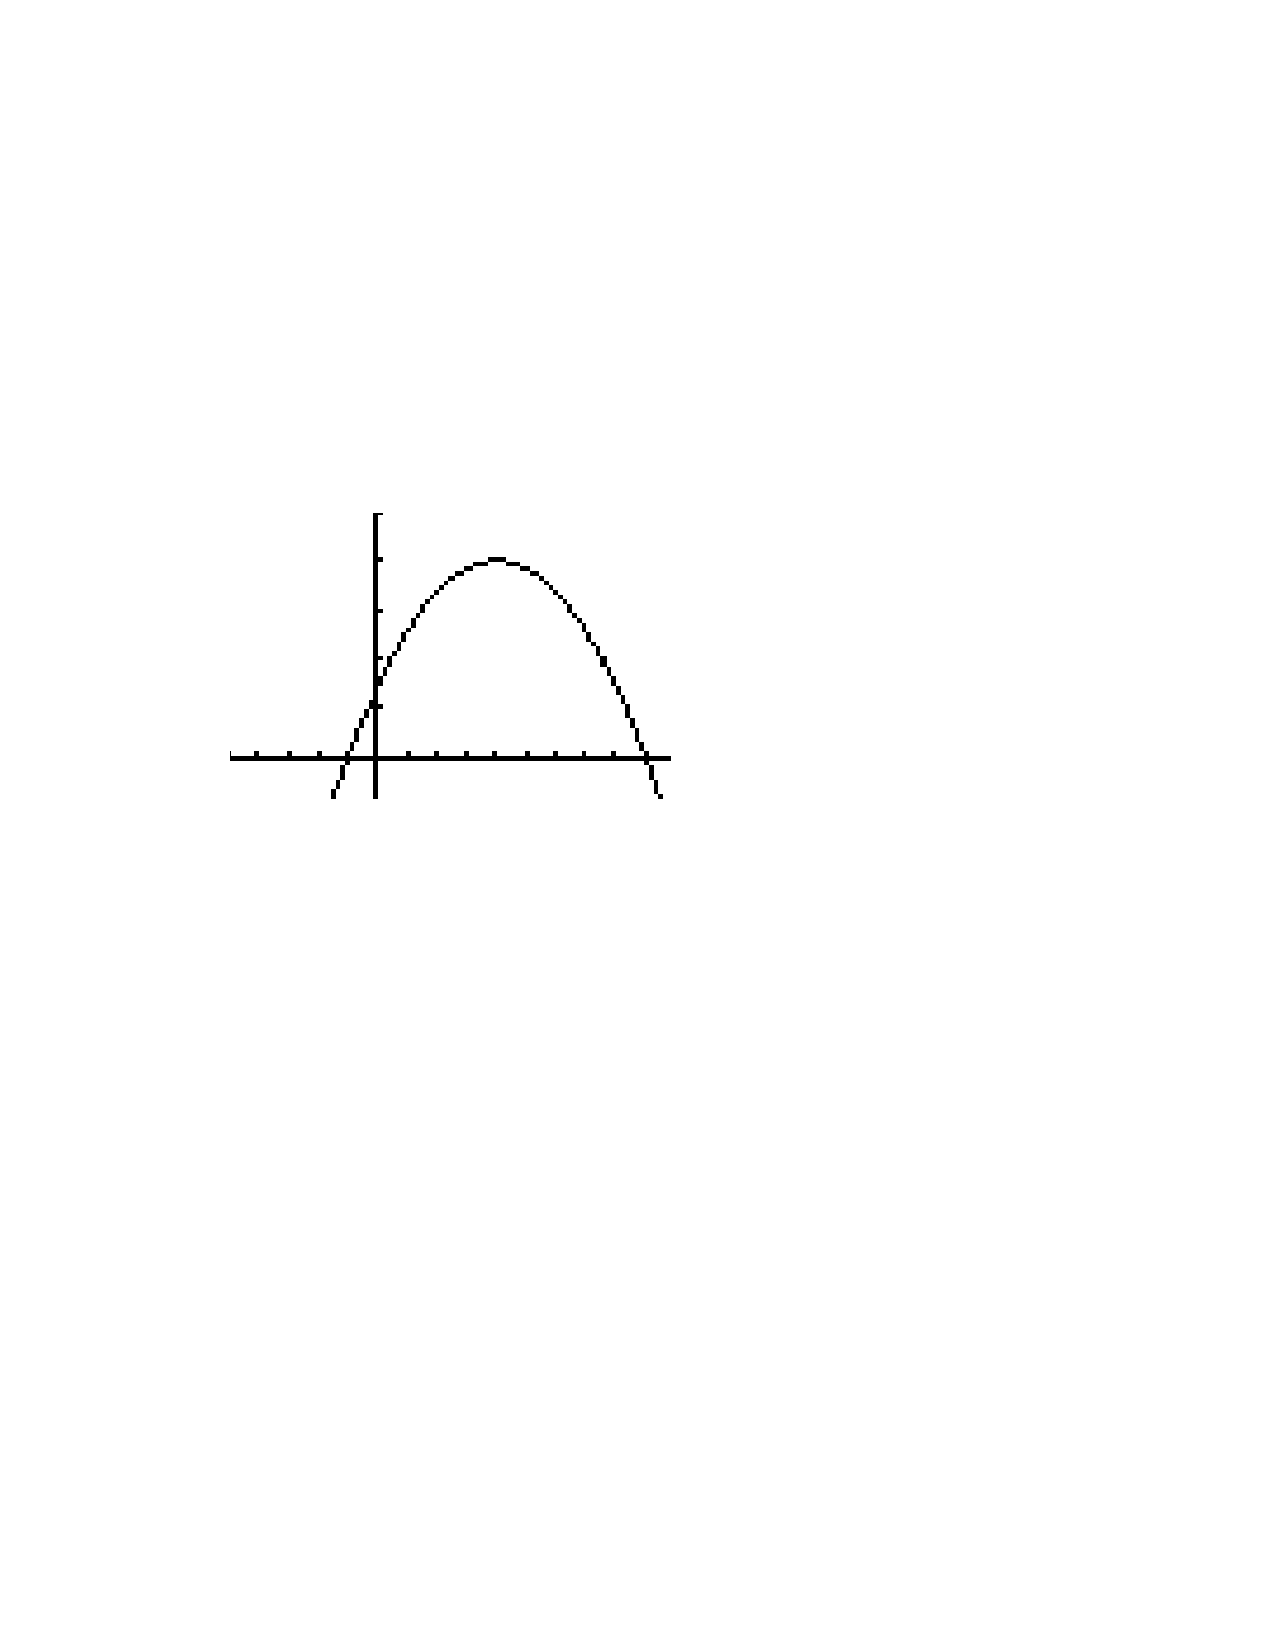
\includegraphics[trim= 170 420 250 180]{Figure1.pdf}
			\end{image}
		\end{freeResponse}	
		
		
	
	%part b	
	\item  True or False:  A moving object can have negative acceleration and increasing speed.

		\begin{freeResponse}
		True.  If your velocity is negative (which means that you are moving in the negative direction) then a negative acceleration increases the magnitude (or absolute value) of the velocity.  But the magnitude of the velocity is the speed.
		\end{freeResponse}	
		
		
		
	\end{enumerate}
	
	
	
	
	

\section*{Group work:}



%problem 1
\begin{problem}
The graph of $s=f(t)$ is the position of an object moving along a number line.
	\begin{image}
	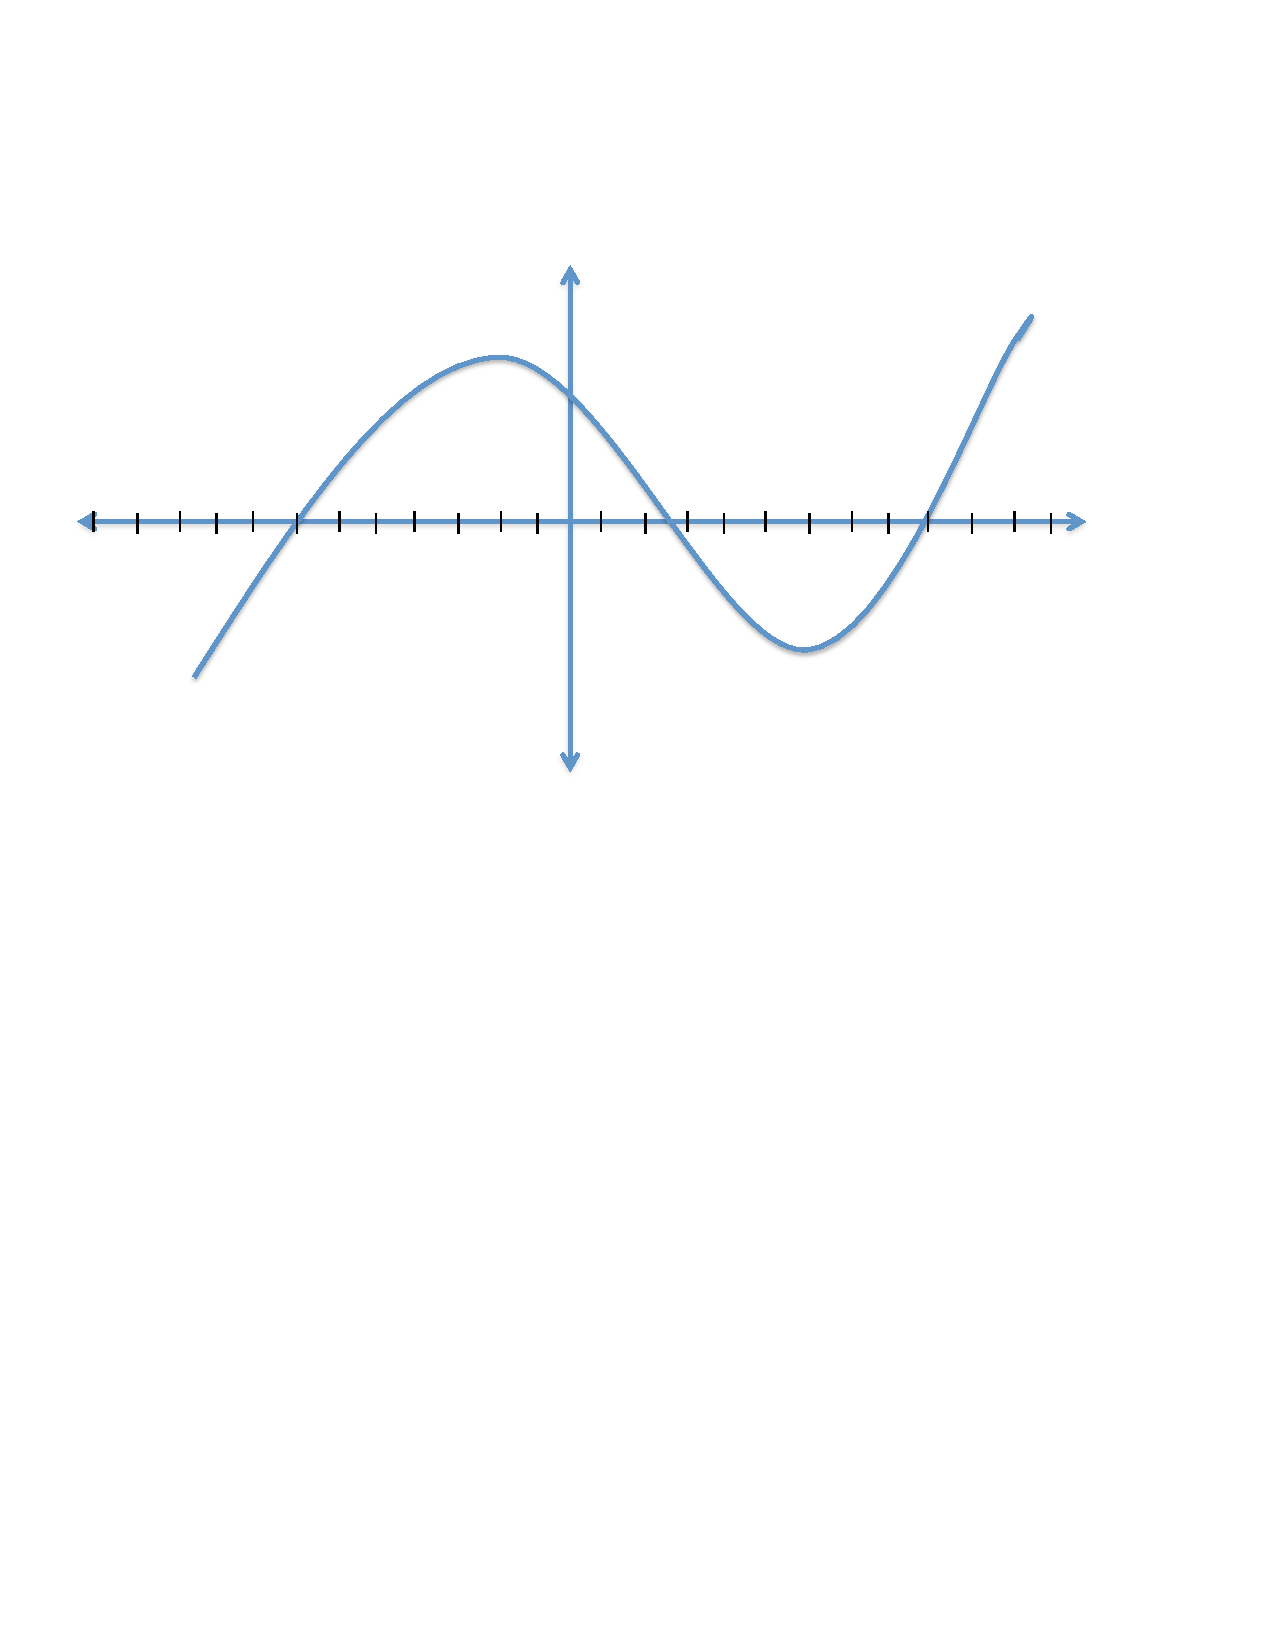
\includegraphics[trim= 140 420 290 180]{Figure2.pdf}
	\end{image}
	
	\begin{enumerate}
	
	%part a
	\item  Describe the motion of the object as precisely as you can.
		\begin{freeResponse}
		Let us assume that $f(t)$ gives the position of John from his house at time $t$.  If $f(t) < 0$, then John is west of his house;  if $f(t) > 0$, then John is east of his house; if $f(t)=0$, then John is in front of his house.  
		
		For the first hour, that is, for $0 \leq t \leq 1$, John walks east away from his house.
		
		\begin{image}
		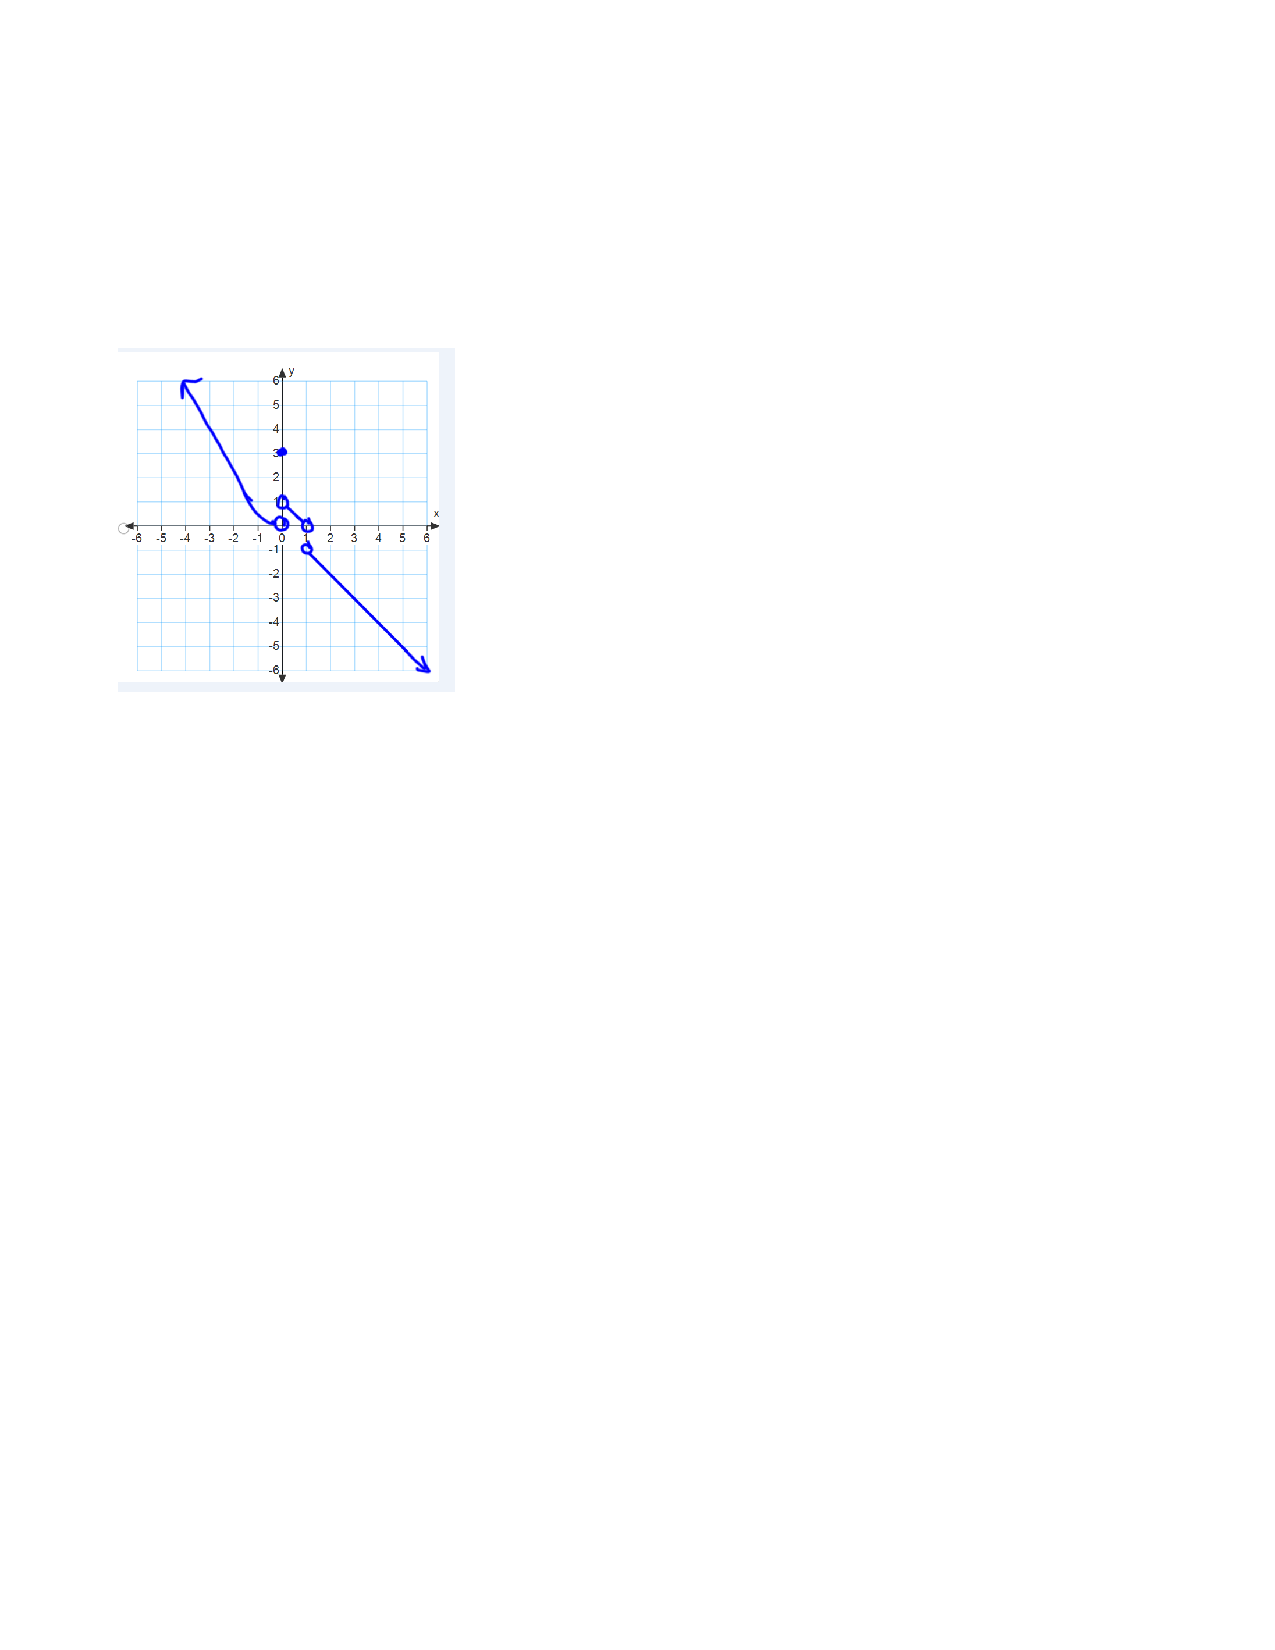
\includegraphics[trim= 140 570 290 200]{Figure3.pdf}
		\end{image}
	
		For the second hour, that is, for $1 \leq t \leq 2$, John turns around and starts walking back west.  However, he does not walk all the way back to his house.
		
		\begin{image}
		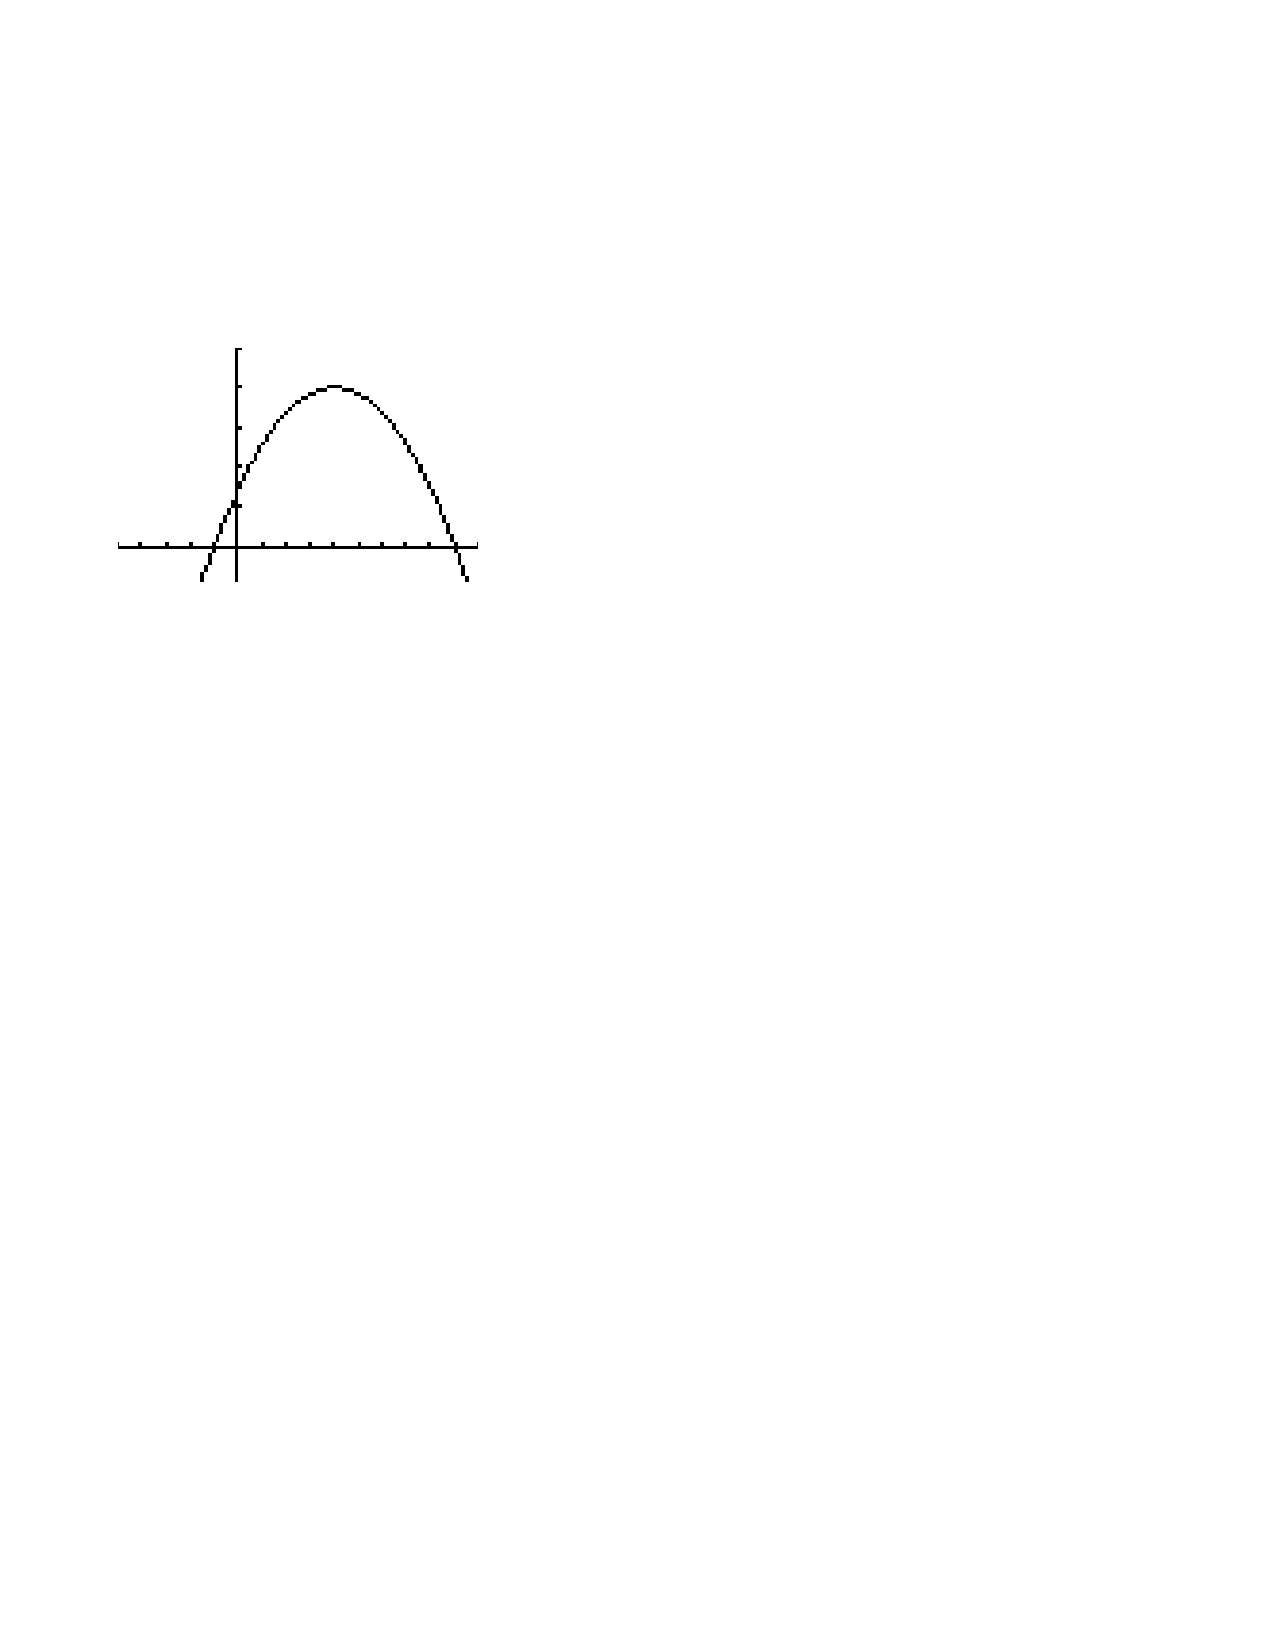
\includegraphics[trim= 140 570 290 200]{Figure4.pdf}
		\end{image}
		
		For the third hour, that is, for $2\le t\le 3$, John realizes he needs to pick up an apple from the grocery store, which is way east of his house, for Elaine.  So he turns around again and walks east to the store.
		
		\begin{image}
		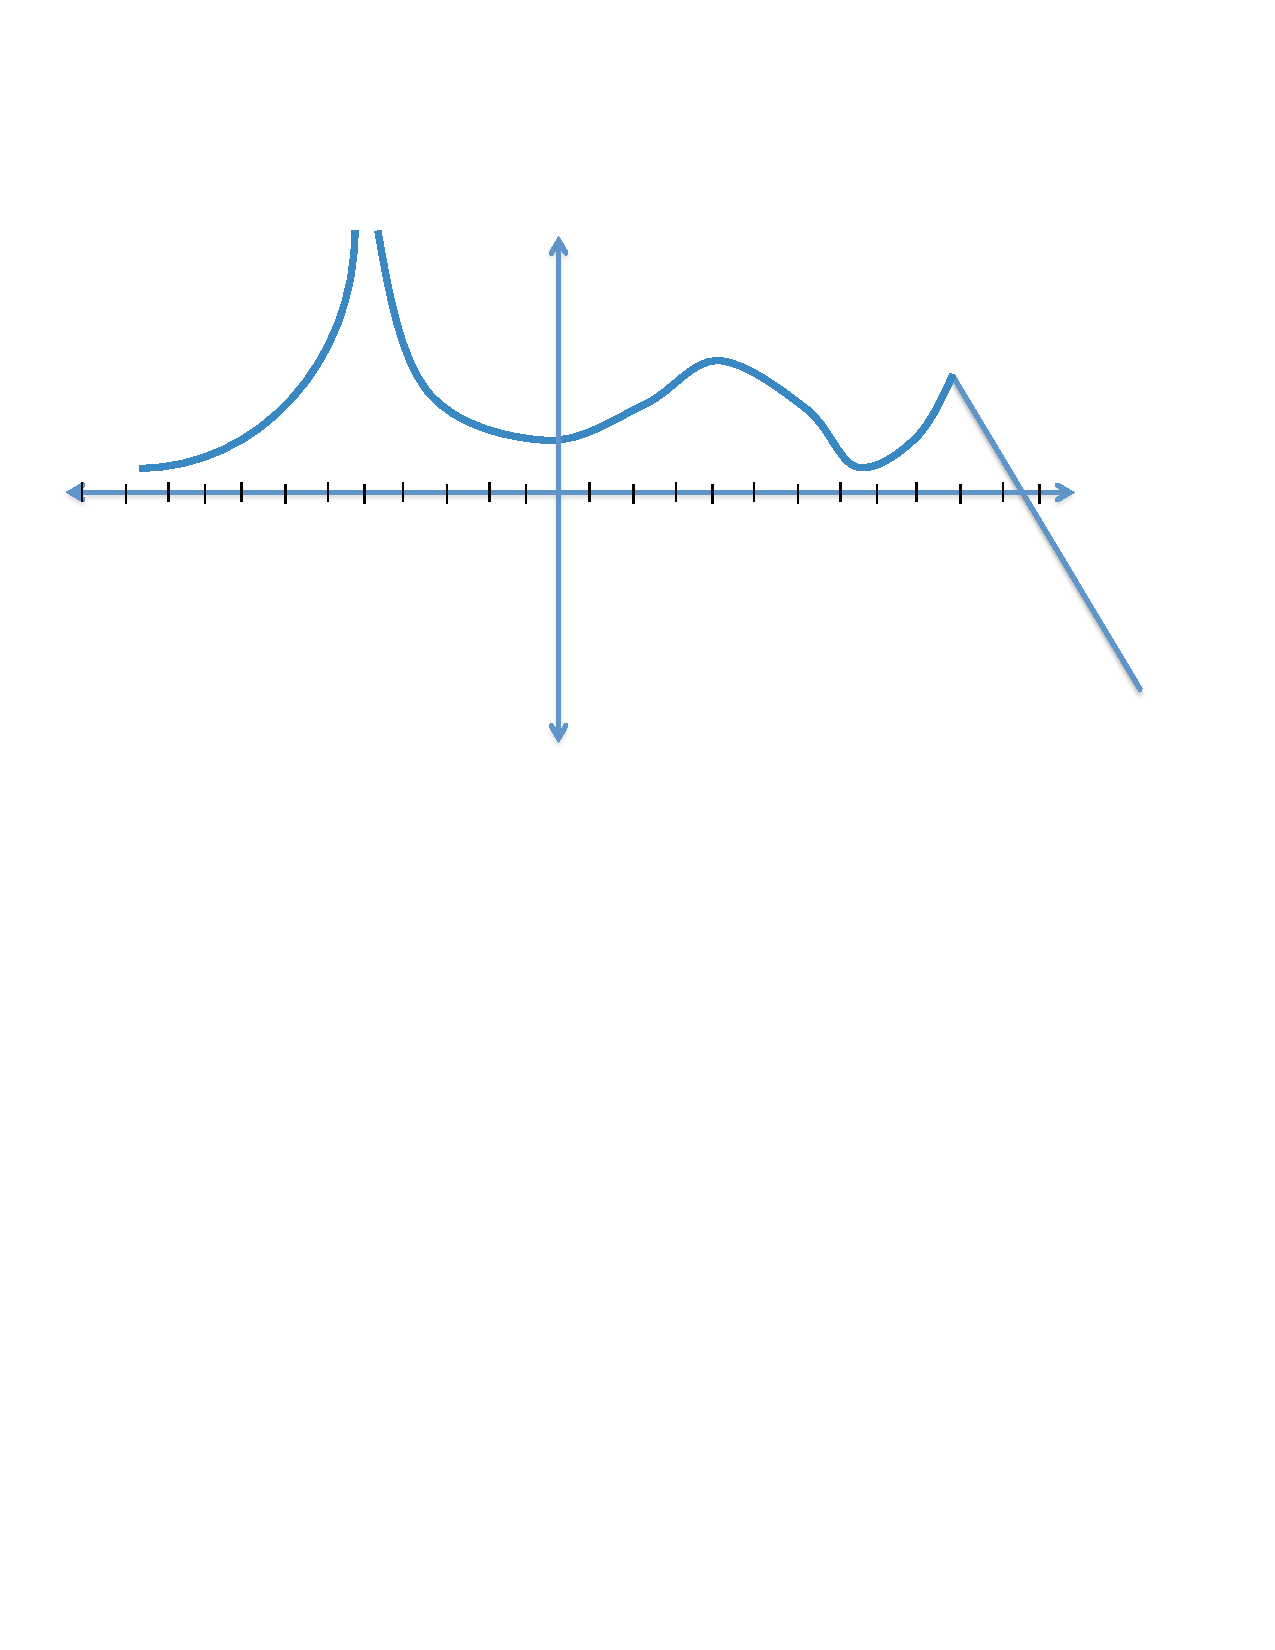
\includegraphics[trim= 140 570 290 200]{Figure5.pdf}
		\end{image}
		
		For the fourth hour, that is, for $t \ge 3$, John needs to drop the apple off at Elaine's house, which is west of his house.  He turns west and walks past his house until he makes it to Elaine's house.
		
		\begin{image}
		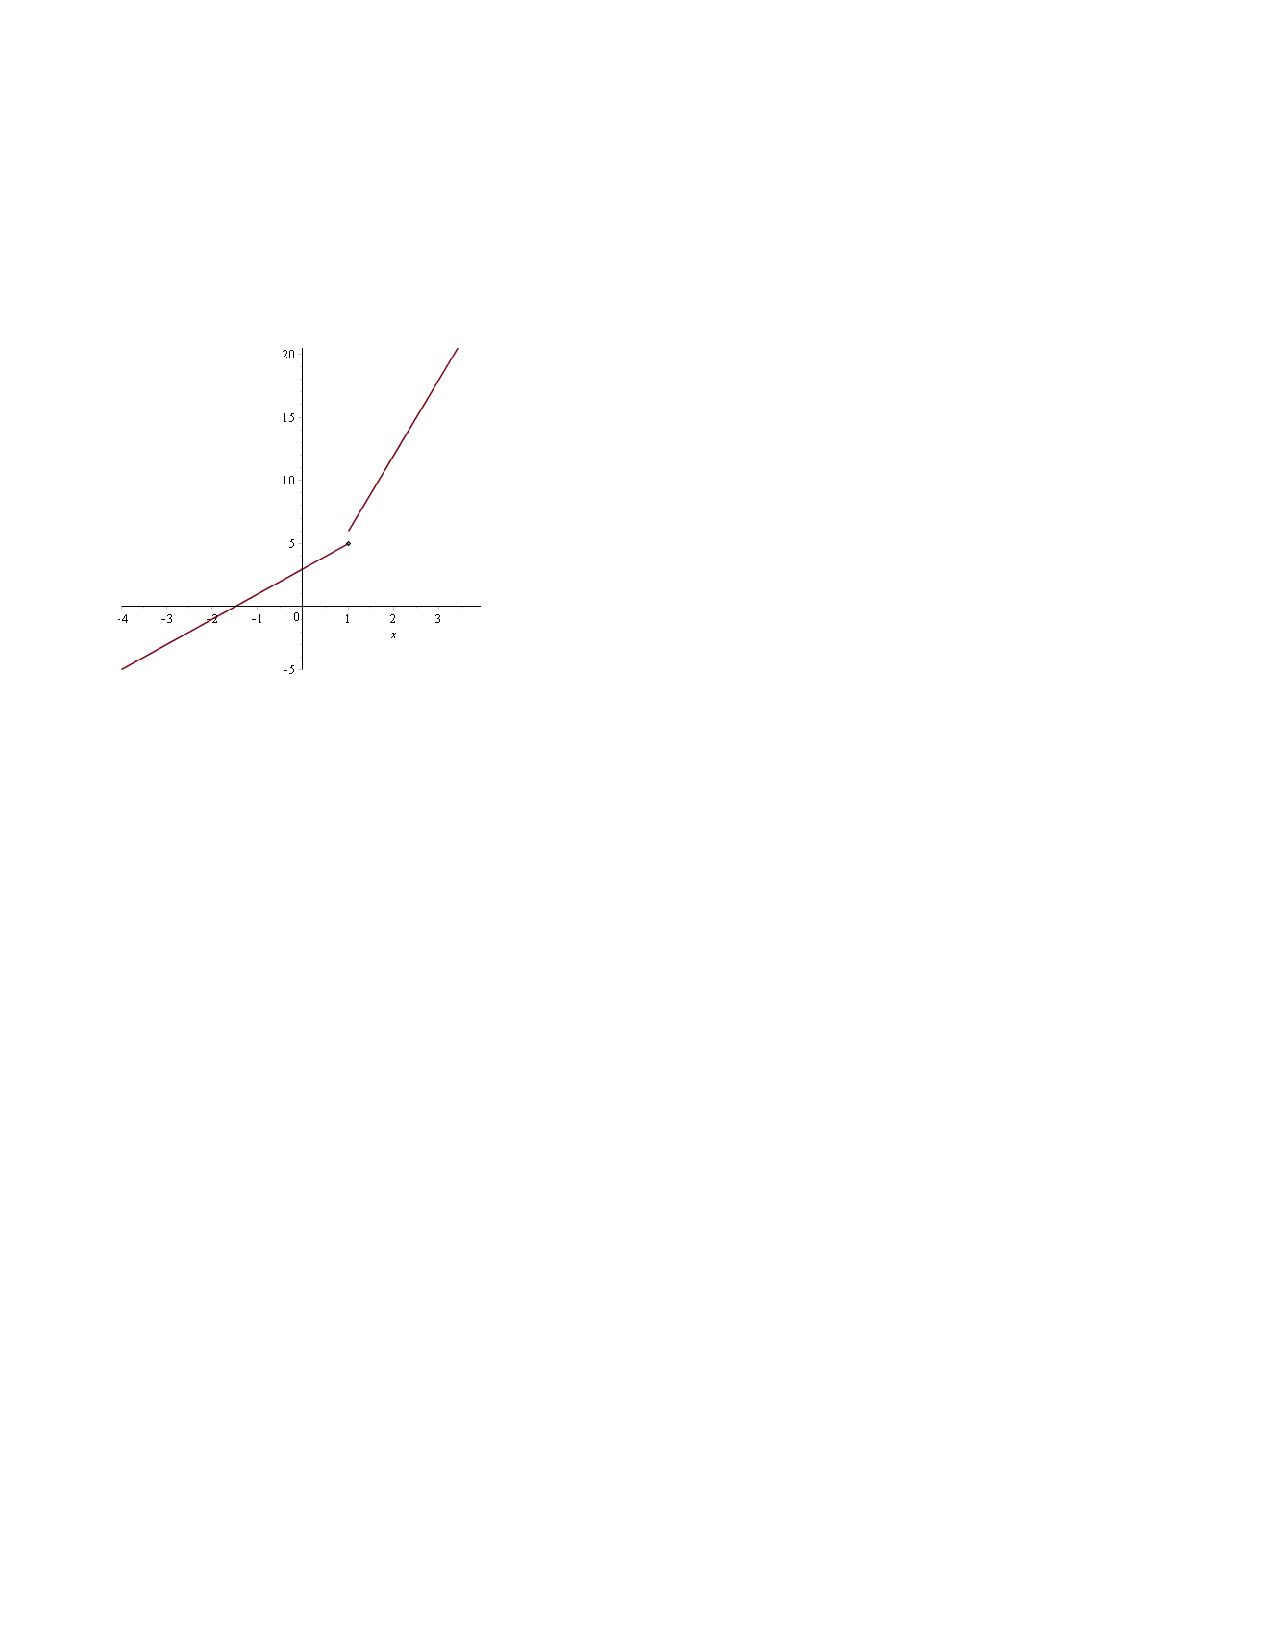
\includegraphics[trim= 140 540 290 200]{Figure6.pdf}
		\end{image}

		\end{freeResponse}
		
		
		
	%part b
	\item  When is the velocity of the object zero?  What is happening to the object at those times? 
		\begin{freeResponse}
		John's velocity is zero at times $t=0,t=1,t=2$, and $t=3$ (the times where the slopes of the tangent lines are zero).  At these times, John changes direction since the slopes of the tangent lines to the graph of $f(t)$ change from positive to negative.
		\end{freeResponse}
		
		
		
	%part c
	\item  When is the object moving in the positive direction?  When is the object the furthest in the positive direction and the furthest in the negative direction?
		\begin{freeResponse}
		John is moving in the positive direction (in this story, east) during times in the region $(0,1) \cup (2,3)$.  John is furthest in the positive direction at time $t=3$ and furthest in the negative direction at (approximately) time $t=3.5$.
		\end{freeResponse}
		
		
		
	%part d
	\item  When is the object speeding up and slowing down? When is the object going at maximum velocity?
		\begin{freeResponse}
		John is speeding up in the region $(0,0.5) \cup (1, 1.5) \cup (2, 2.5) \cup (3, 3.5)$.  He is slowing down in the region $(0.5, 1) \cup (1.5, 2) \cup (2.5, 3)$.  John is moving the fastest at time $t = 3.5$, but that maximizes his speed, not his velocity, because he is moving in the negative direction at that time.  It appears that he maximizes his velocity at about $t=2.5$.  
		\end{freeResponse}
		
		
		
	\end{enumerate}
			
			
	
\end{problem}
















%problem 2
\begin{problem}
Suppose that a stone is thrown vertically upward from a cliff on Mars with an initial velocity of $64$ ft/s from a height of $192$ ft.  The height $s$ of the stone above the ground after $t$ seconds is given by $s(t) = -6t^2 + 24t + 192$.

	\begin{enumerate}
	
	%part a
	\item  Determine the velocity and acceleration of the stone after $t$ seconds.
			\begin{freeResponse}
			The velocity $v(t)$ is:  $v(t) = s'(t) = -12t + 24$.
			
			The acceleration $a(t)$ is:  $a(t) = v'(t) = s''(t) = -12$.
			\end{freeResponse}
			
			
			
	%part b
	\item  What is the greatest height of the stone and when does it occur?  What are the velocity and acceleration at that time?
			\begin{freeResponse}
			Since the function $s(t)$ is differentiable everywhere (it is a polynomial), the maximum height must occur at a time when the velocity is $0$.  So we solve:
			\begin{align*}
			v(t) = -12t+24 &:= 0 \\
			12t &= 24 \\
			t &= 2
			\end{align*}
			
			It is easy to check that $v(t) > 0$ for $0 \leq t < 2$ and $v(t) < 0$ for $2 < t$, and so the greatest height of the stone really does occur at time $t=2$.  The greatest height is $s(2) = -24 + 48 + 192 = 216$ ft.  For the second question we have already seen that $v(2) = 0$ ft/sec, and we have a constant acceleration of $-12$ ft/sec$^2$.  So $a(2) = -12$ ft/sec$^2$.
			\end{freeResponse}
			
			
			
	%part c
	\item  When does the stone hit the ground?  What are the velocity and acceleration at that time?
			\begin{freeResponse}
			The stone hits the ground when $s(t) = 0$.  So we solve:
			\begin{align*}
			s(t) = -6t^2 + 24t + 192 &:= 0 \\
			-6(t^2 - 4t - 32) &= 0 \\
			-6(t-8)(t+4) &= 0 
			\end{align*}
			
			Since we are only considering $t \geq 0$, we must have $t=8$.  At this instant, $v(8) = -96 + 24 = -72$ ft/sec and $a(8) = -12$ ft/sec$^2$.  
			
			\end{freeResponse}
			
			
			
	\end{enumerate}
			
			
			
		
\end{problem}
	
	
	
	
	
	
	
	
			
			








	
	
	
	
	
	
	
	
	

	










								
				
				
	














\end{document} 


















